\documentclass[border=0.8ex,svgnames,tikz]{standalone}
\usepackage{amsmath,mathtools}
\usepackage{fontspec}
\setmainfont{Source Serif 4}
\setsansfont{Source Sans 3}
\setmonofont{Source Code Pro}
\usepackage{ctex}
\setCJKmainfont[BoldFont=Source Han Sans CN]{Source Han Serif CN}
\usetikzlibrary{positioning}
\begin{document}
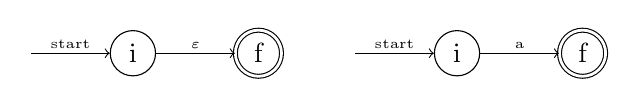
\begin{tikzpicture}
  % \varepsilone
  \node[text width=-3em](EpsilonStart){};
  \node[circle, draw=black, right= of EpsilonStart](EpsilonI){i};
  \node[circle, double, double distance=1pt, draw=black, right= of EpsilonI](EpsilonF){f};
  \path[->]
  (EpsilonStart) edge node[above=-2pt]{\tiny start} (EpsilonI)
  (EpsilonI) edge node[above=-2pt]{\tiny $\varepsilon$} (EpsilonF);

  % subexpr a
  % \node[text width=-3em, below=1.25em of EpsilonStart](SubExprStart){};
  \node[text width=-3em, right=2.5em of EpsilonF](SubExprStart){};
  \node[circle, draw=black, right= of SubExprStart](SubExprI){i};
  \node[circle, double, double distance=1pt, draw=black, right= of SubExprI](SubExprF){f};
  \path[->]
  (SubExprStart) edge node[above=-2pt]{\tiny start} (SubExprI)
  (SubExprI) edge node[above=-2pt]{\tiny a} (SubExprF);
\end{tikzpicture}
\end{document}
